\documentclass{journal}
%\documentclass[journal]{new-aiaa} for journal papers
\usepackage{graphicx}
\usepackage{amsmath}
\usepackage{amssymb}
\usepackage[version=4]{mhchem}
\usepackage{siunitx}
\usepackage{longtable,tabularx}
\setlength\LTleft{0pt} 

\title{AIRFOIL ANALYSIS}

\author{Nathan Pettit}


\begin{document}
	
	\maketitle	
	
	\section{Introduction}
	This report reviews research done on airfoils. There are 5 areas that are covered in this research. One, it explores the effect of airfoil angle of attack on lift, drag, and moment. Two, it compares data collected by Xfoil to experimental data. Three, it explores the effect of different Reynold's numbers on airfoil polar. Four, it explores the effect of different airfoil thicknesses. And four, it explores the effect of different airfoil cambers.
	
	\section{Methods}
	The results of this research came from evaluating airfoils using Xfoil functions in Julia, as well as writing new functions to help in evaluating the airfoils. There were 4 functions that were  used:
	
	\begin{enumerate}
		\item alterThicknessCamber() - this evaluated airfoils of varying thicknesses and cambers and plotted their lifts and drags together in order to compare them
		\item getCoefficients() - this was a helper function that was used to calculate the coefficients of lift, drag, and moment and return them to other functions that needed those calculations done
		\item alterReynolds() - this evaluated an airfoil using varying Reynold's numbers and plotted their lift, drag, and moment in order to compare them
		\item autoSweep() - this calculated and plotted an airfoil's lift, drag, and moment with varying airfoil angles of attack
	\end{enumerate}
	
	\section{Results and Discussion}
	
	\subsection{Airfoil Angle  of Attack}
	One of the most stressed parts of this research was seeing how different airfoil angles of attack affected the lift, drag, and moment on the airfoil. In order to see those relationships, only the coefficients of drag, lift, and moment needed to evaluated, rather than the moment and the forces of lift and drag. This is because in calculating lift, drag, and moment, the only parts that differ are the coefficients. Figure \ref{fig:aoa-coefficients} shows the relationships between lift, drag, and moment and \(\alpha\) for a NACA 2412 airfoil.
	
	\begin{figure}
		\centering
		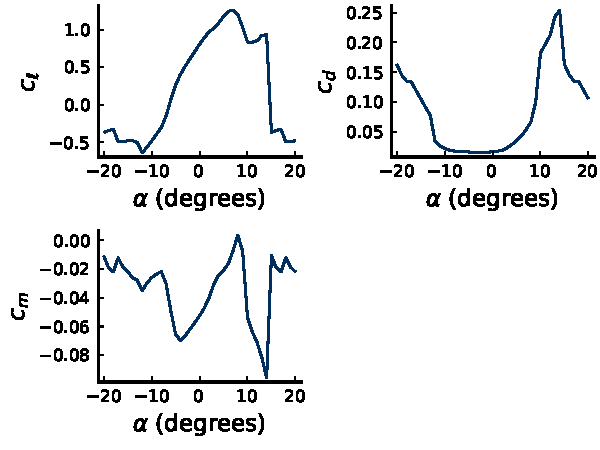
\includegraphics{../graphics/aoa-coefficients.pdf}
		\caption{\emph{coefficients of lift, drag, and moment plotted against angle of attack for a NACA 2412 airfoil}}
		\label{fig:aoa-coefficients}
	\end{figure}
	
	The coefficients of lift (\(c_\ell\)) and drag (\(c_d\)) both increase as angle of attack (\(\alpha\)) increases, because as the angle increases, the area of the airfoil going against the fluid increases, and the pressure acting on the bottom of the airfoil also increases. This also increases coefficient of moment (\(c_m\)). It is also important to note that figure \ref{fig:aoa-coefficients} establishes that lift is negative when \(\alpha\) is less than zero, which makes sense, and that the zero-lift angle of attack is somewhere between 0 and 0.5 degrees. Stall is also something to be aware of, but the figure doesn't indicate this as stalling would take place with angles that are greater than 10 degrees.
	
	\subsection{Airfoil Polar Comparison}
	The results gained from Xfoil were plotted against experimental data from a study done on the NACA 2412 airfoil (see figure \ref{fig:airfoil-comparison}).
	
	\begin{figure}
		\centering
		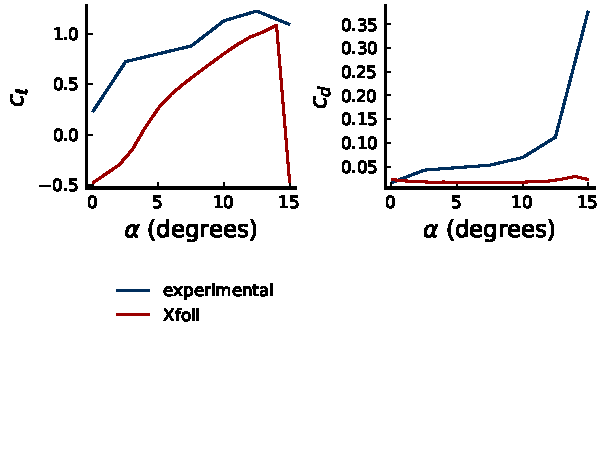
\includegraphics{../graphics/airfoil-compare.pdf}
		\caption{\emph{comparison of data collected experimentally to data collected from Xfoil}}
		\label{fig:airfoil-comparison}
	\end{figure}

	The data collected from Xfoil followed the experimental data's curve, therefore, it is an accurate way to model airfoil polar.
	
	\subsection{Effect of Reynold's Number}
	The Reynold's number is an indicator of how viscous the fluid that an airfoil is traveling through is. A high Reynold's number is an indicator that fluid flow will be turbulent, where as a low Reynold's number is an indicator of laminar flow. In figure \ref{fig:altered-reynolds}, the relationships between Reynold's number and the coefficients are shown.
	
	\begin{figure}
		\centering
		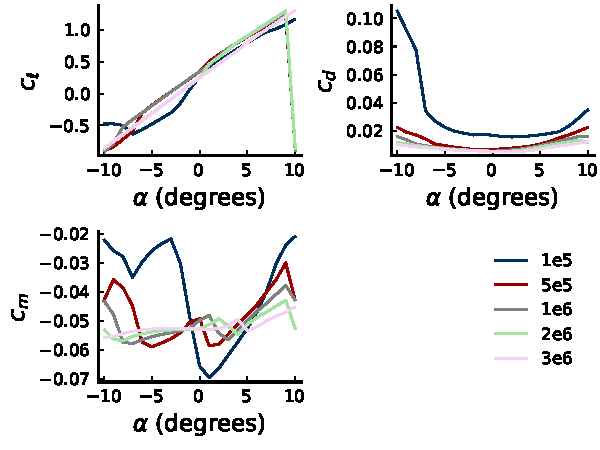
\includegraphics{../graphics/altered-reynolds.pdf}
		\caption{\emph{plots of lift, drag, and moment for varying Reynold's numbers}}
		\label{fig:altered-reynolds}
	\end{figure}
	
	As the Reynold's number increases, the lift curves become more steep. However, it is the opposite with drag and moment. As the Reynold's number increases, the curves of drag and moment become more leveled out. These results make logical sense, because whether with turbulent or laminar flow, lift generally is not affected significantly across varying angles of attack. On the other hand, higher Reynold's numbers and therefore more turbulent flow decreases the drag and moment at more extreme angles of attack (see figure \ref{fig:altered-reynolds}).
	
	\subsection{Effect of Airfoil Thickness and Camber}
	The thickness of an airfoil is the greatest distance between the upper and the lower surfaces of an airfoil. In figure \ref{fig:altered-thickness}, the relationship between airfoil thickness and the coefficients of lift, drag, and moment can be seen.
	
	\begin{figure}
		\centering
		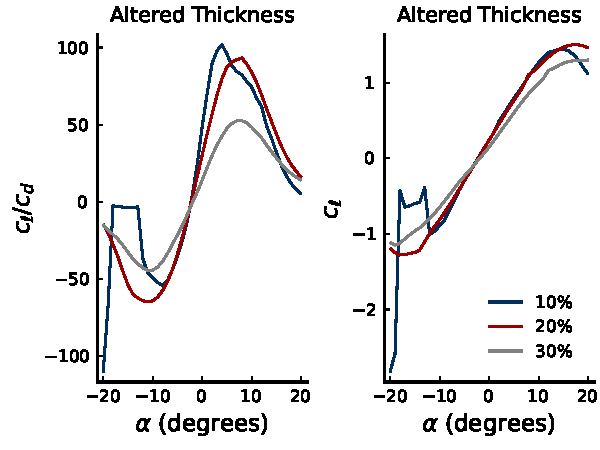
\includegraphics{../graphics/altered-thickness.pdf}
		\caption{\emph{plots of ratio of lift to drag coefficients and coefficient of lift}}
		\label{fig:altered-thickness}
	\end{figure}
	
	As the thickness of the airfoil increases, the ratio of lift to drag curve becomes more shallow. This is because increasing thickness leads to lift and drag becoming closer and closer to each other. It is interesting to see though that no matter the thickness, the zero lift angle of attack remains the same (see figure \ref{fig:altered-thickness}).
	
	The camber of an airfoil is the asymmetry between the two acting surfaces of an airfoil. An airfoil with zero camber is symmetric. In figure \ref{fig:altered-camber}, the effect of different cambers can be seen.
	
	\begin{figure}
		\centering
		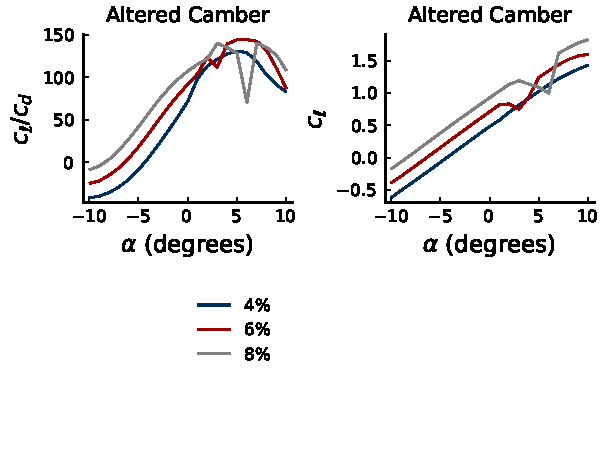
\includegraphics{../graphics/altered-camber.pdf}
		\caption{\emph{plots of ratio of lift to drag coefficients and coefficient of lift}}
		\label{fig:altered-camber}
	\end{figure}
	
	As the camber of the airfoil increases, the lift to drag ratio becomes higher and the whole curve is shifted upwards. This also happened with the coefficient of lift. This also means that the zero lift angle of attack became greater with increasing camber. 
	
	
	\section*{Appendix}
	
	\begin{itemize}
		\item Irrotational flow: a flow in which each element of the moving fluid undergoes no net rotation with respect to a chosen coordinate axes from one instant to other
		\item Inviscid: having no or negligible viscosity
		\item Chord: a straight line from the leading edge to the trailing edge (see figure \ref{fig:airfoil-diagram})
		\item Airfoil camber: the asymmetry between the two acting surfaces of an airfoil, with the top surface of a wing commonly being more convex. An airfoil that is not cambered is called a symmetric airfoil (see figure \ref{fig:airfoil-diagram})
		\item Airfoil thickness: the greatest distance between the upper and the lower surfaces of an airfoil (see figure \ref{fig:airfoil-diagram})
		
		\begin{figure}
			\centering
			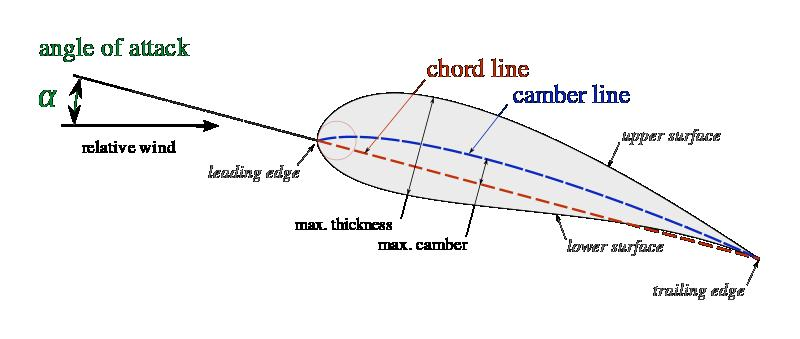
\includegraphics[scale=0.4]{../graphics/airfoil-diagram.jpg}
			\caption{\emph{airfoil diagram showing angle of attack, airfoil camber, thickness, and chord}}
			\label{fig:airfoil-diagram}
		\end{figure}
		
		\item Potential flow: an idealized model of fluid flow that occurs in the case of incompressible, inviscid, and irrotational flow
		\item Freestream: the air far upstream of an aerodynamic body, that is, before the body has a chance to deflect, slow down or compress the air
		\item Angle of attack: the angle at which the chord of an aircraft's wing meets the relative wind
		\item Drag coefficient: equal to the drag D divided by density r times half the velocity V squared times the reference area A. It expresses the ratio of the drag force to the force produced by the dynamic pressure times the area (see equation \ref{eqn:drag})
		
		\begin{equation}
			\centering
			\label{eqn:drag}
			c_d = \frac{2D}{\rho{V^2}S}
		\end{equation}
	
		\item Lift coefficient: relates the lift generated by a lifting body to the fluid density around the body, the fluid velocity and an associated reference area (see equation \ref{eqn:lift})
		
		\begin{equation}
			\centering
			\label{eqn:lift}
			c_\ell = \frac{2L}{\rho{V^2}S}
		\end{equation}
	
		\item Moment coefficient: pertains to the moment specifically due to the aerodynamics force (see equation \ref{eqn:moment})
		
		\begin{equation}
			\centering
			\label{eqn:moment}
			c_m = \frac{2M}{\rho{V^2}S}
		\end{equation}
	
		\item Stall: a sudden reduction in the lift generated by an aerofoil when the critical angle of attack is reached or exceeded	
		\item Airfoil polar: represent the aerodynamic characteristics of an airfoil (figure \ref{fig:aoa-coefficients} is an example of an airfoil polar)
		\item Reynold's number: helps predict flow patterns in different fluid flow situations. At low Reynolds numbers, flows tend to be dominated by laminar (sheet-like) flow, while at high Reynolds numbers flows tend to be turbulent. Equation \ref{eqn:velocity} calculates Reynold's number using \(\rho\)(density), u(flow speed), L(characteristic linear dimension), and \(\mu\)(dynamic viscosity of fluid)
		
		\begin{equation}
			\centering
			\label{eqn:velocity}
			R_e = \frac{\rho{uL}}{\mu}
		\end{equation}
		
		\item Mach number: ratio of the speed of a body to the speed of sound in the surrounding medium
		\item Lift curve slope: measure of how rapidly the wing generates lift with change in AOA (see figure \ref{fig:lift-curve-slope})
		
		\begin{figure}
			\centering
			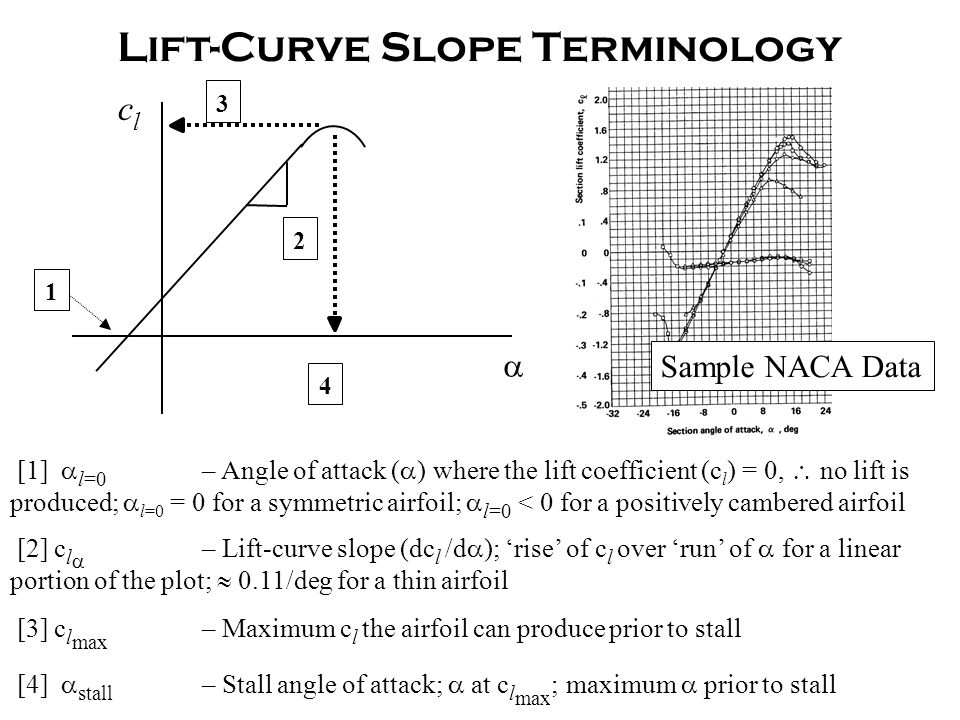
\includegraphics[scale=0.4]{../graphics/lift-curve-slope.jpg}
			\caption{\emph{This diagram shows the major characteristics of a lift curve}}
			\label{fig:lift-curve-slope}
		\end{figure}
	
	\end{itemize}
	
	
\end{document}